\documentclass[12pt, a4paper]{article}
\usepackage[utf8]{inputenc}
\usepackage[T2A]{fontenc}
\usepackage[russian]{babel}
\usepackage{graphicx}
\usepackage{amsmath}
\usepackage{geometry}
\geometry{top=2cm, bottom=2cm, left=3cm, right=1.5cm}

\begin{document}

\begin{titlepage}
    \begin{center}
        \Large \textbf{МИНИСТЕРСТВО НАУКИ И ВЫСШЕГО ОБРАЗОВАНИЯ РОССИЙСКОЙ ФЕДЕРАЦИИ} \\
        \vspace{1cm}
        \large Московский авиационный институт \\
        (национальный исследовательский университет) \\
        \vspace{2cm}
        \Large \textbf{Отчёт по лабораторной работе №2} \\
        \vspace{0.5cm}
        \large \textbf{«Управление процессами и межпроцессное взаимодействие»} \\
        \vspace{3cm}
        \begin{flushright}
            \normalsize
            \textbf{Выполнила:} студентка группы М8О-203БВ-25 \\
            Петрова Эвелина \\
            \textbf{Вариант:} 17 \\
        \end{flushright}
        \vfill
        \large \textbf{Москва, 2026}
    \end{center}
\end{titlepage}

\newpage
\tableofcontents
\newpage


\section{Цель работы}
Приобретение практических навыков в управлении процессами в операционной системе и обеспечении обмена данными между процессами посредством каналов (pipe).

\section{Задание}
Составить и отладить программу, осуществляющую работу с процессами и взаимодействие между ними в операционной системе Linux. В результате работы программа должна создать для решения задачи два дочерних процесса. Взаимодействие между процессами осуществляется через неименованные каналы (pipe). Необходимо обрабатывать системные ошибки, которые могут возникнуть в результате работы.

\textbf{Вариант 17 (Группа вариантов 5):} Родительский процесс создает два дочерних процесса. Первой строкой пользователь в консоль родительского процесса вводит имя файла, которое будет использовано для открытия файла с таким именем на запись для child1. Аналогично для второй строки и процесса child2. Родительский и дочерний процесс должны быть представлены разными программами.

Родительский процесс принимает от пользователя строки произвольной длины и пересылает их в pipe1 или в pipe2 в зависимости от правила фильтрации. Процесс child1 и child2 производят работу над строками. Процессы пишут результаты своей работы в стандартный вывод.

\textbf{Правило фильтрации:} строки длины больше 10 символов отправляются в pipe2, иначе в pipe1. Дочерние процессы удаляют все гласные из строк.

Схема межпроцессного взаимодействия приведена на рисунке 1.

\begin{figure}[h!]
    \centering
    \fbox{
        \begin{minipage}{0.8\textwidth}
            \centering
            \textbf{Схема взаимодействия (Вариант 17)} \\
            \vspace{0.5cm}
            Parent $\rightarrow$ pipe1 $\rightarrow$ Child1 $\rightarrow$ stdout \\
            Parent $\rightarrow$ pipe2 $\rightarrow$ Child2 $\rightarrow$ stdout \\
            Child1 $\rightarrow$ file1 (out1.txt) \\
            Child2 $\rightarrow$ file2 (out2.txt)
        \end{minipage}
    }
    \caption{Схема межпроцессного взаимодействия}
    \label{fig:scheme}
\end{figure}

% === ТЕОРЕТИЧЕСКИЕ СВЕДЕНИЯ ===
\section{Теоретические сведения}

\subsection{Системные вызовы в ОС Linux}
Для реализации межпроцессного взаимодействия в POSIX-системах (Linux) используются следующие системные вызовы:

\begin{itemize}
    \item \texttt{pid\_t fork()} --- создание дочернего процесса. Дочерний процесс является точной копией родителя и наследует все его файловые дескрипторы. Возвращает 0 в дочернем процессе и PID дочернего в родительском.
    
    \item \texttt{int execve(const char *filename, char *const argv[], char *const envp[])} (и другие вариации \texttt{exec}) --- замена образа памяти процесса. После успешного вызова текущая программа заменяется новой.
    
    \item \texttt{pid\_t waitpid(pid\_t pid, int *status, int options)} --- ожидание завершения дочернего процесса. Блокирует вызывающий процесс до тех пор, пока указанный дочерний процесс не завершится.
    
    \item \texttt{void exit(int status)} --- завершение выполнения процесса и возвращение статуса.
    
    \item \texttt{int pipe(int pipefd[2])} --- создание неименованного канала для передачи данных между процессами. \texttt{pipefd[0]} --- дескриптор для чтения, \texttt{pipefd[1]} --- для записи.
    
    \item \texttt{int dup2(int oldfd, int newfd)} --- переназначение файлового дескриптора. Используется для перенаправления стандартного ввода/вывода на канал.
    
    \item \texttt{int open(const char *pathname, int flags, mode\_t mode)} --- открытие/создание файла.
    
    \item \texttt{int close(int fd)} --- закрыть файловый дескриптор.
\end{itemize}

\subsection{Системные вызовы в ОС Windows}
Для полноты описания кроссплатформенного решения приводятся аналогичные вызовы Windows API:

\begin{itemize}
    \item \texttt{BOOL WINAPI CreateProcess(...)} --- создание нового процесса.
    \item \texttt{WaitForSingleObject(...)} --- ожидание завершения процесса.
    \item \texttt{ExitProcess(...)} --- завершение выполнения процесса.
    \item \texttt{CreatePipe(...)} --- создание безымянного канала.
    \item \texttt{CreateFile(...)} --- создание нового файла.
    \item \texttt{CloseHandle(...)} --- закрытие объекта ОС.
\end{itemize}

\subsection{Проблема наследования файловых дескрипторов}
Ключевой особенностью системного вызова \texttt{fork()} является то, что дочерний процесс наследует \textit{все} открытые файловые дескрипторы родителя. Это означает, что если родитель создал два канала (pipe1 и pipe2), то каждый дочерний процесс получит копии дескрипторов обоих каналов.

Если дочерний процесс не закроет явно дескрипторы «чужого» канала (того, который ему не предназначен), то при закрытии write-end канала родительским процессом чтение из read-end никогда не вернёт признак конца файла (EOF), поскольку ядро ОС считает канал открытым, пока хотя бы один процесс держит write-end открытым. Это приводит к взаимной блокировке (deadlock): дочерний процесс бесконечно ожидает данные, а родительский процесс бесконечно ожидает завершения дочернего через \texttt{waitpid()}.

\section{Описание программы}

\subsection{Структура проекта}
Проект имеет модульную кроссплатформенную структуру:

\begin{itemize}
    \item \texttt{common/} --- общие утилиты: определения платформы (\texttt{defines.h}), функции логирования (\texttt{errors.h}, \texttt{errors.cpp}).
    
    \item \texttt{os/} --- абстракция над API операционной системы. Содержит объявления классов \texttt{Pipe} и \texttt{ProcessHandle} (\texttt{process.h}), общую бизнес-логику (\texttt{process.cpp}), а также платформенно-зависимые реализации: \texttt{process\_posix.cpp} для Linux и \texttt{process\_win.cpp} для Windows.
    
    \item \texttt{parent/} --- родительский процесс (\texttt{main.cpp}). Отвечает за создание каналов, запуск дочерних процессов, маршрутизацию ввода пользователя и ожидание завершения детей.
    
    \item \texttt{child/} --- дочерний процесс (\texttt{main.cpp}). Читает строки из стандартного ввода (перенаправленного на канал), удаляет гласные буквы и записывает результат в файл и стандартный вывод.
\end{itemize}

Система сборки CMake автоматически выбирает нужную реализацию в зависимости от операционной системы:
\begin{verbatim}
if(WIN32)
    set(OS_SOURCES process.cpp process_win.cpp)
else()
    set(OS_SOURCES process.cpp process_posix.cpp)
endif()
\end{verbatim}

\subsection{Алгоритм работы родительского процесса}
\begin{enumerate}
    \item Запрос у пользователя имён файлов для child1 и child2.
    \item Создание двух неименованных каналов (\texttt{pipe1}, \texttt{pipe2}) через системный вызов \texttt{pipe()}.
    \item Запуск двух дочерних процессов через функцию \texttt{start\_process()}, которая:
    \begin{itemize}
        \item вызывает \texttt{fork()} для создания дочернего процесса;
        \item в дочернем процессе перенаправляет stdin на read-end нужного канала через \texttt{dup2()};
        \item закрывает write-end нужного канала и оба конца «чужого» канала;
        \item вызывает \texttt{execl()} для замены образа процесса программой child.
    \end{itemize}
    \item Чтение строк от пользователя в цикле.
    \item Применение правила фильтрации варианта 17: если длина строки $> 10$ символов --- отправка в \texttt{pipe2} (child2), иначе --- в \texttt{pipe1} (child1).
    \item При получении пустой строки --- закрытие write-end обоих каналов (для передачи EOF дочерним процессам).
    \item Ожидание завершения дочерних процессов через \texttt{waitpid()}.
\end{enumerate}

\subsection{Алгоритм работы дочернего процесса}
\begin{enumerate}
    \item Получение аргументов командной строки: имя выходного файла и идентификатор процесса.
    \item Открытие файла на запись.
    \item Чтение строк из стандартного ввода (который перенаправлен на канал родителем).
    \item Вызов функции \texttt{remove\_vowels()} для удаления всех гласных букв (английских и русских).
    \item Запись результата в файл и стандартный вывод.
    \item Автоматическое завершение при получении EOF (когда родитель закрывает write-end канала).
\end{enumerate}

\subsection{Решение проблемы дедлока}
Проблема взаимной блокировки решена путём явной передачи ссылки на «другой» канал в функцию \texttt{start\_process()}. Дочерний процесс принудительно закрывает оба конца «чужого» канала перед вызовом \texttt{execl()}:

\begin{verbatim}
// В дочернем процессе:
other_pipe.close_read();
other_pipe.close_write();
\end{verbatim}

Это гарантирует, что после закрытия write-end канала родительским процессом, чтение из read-end корректно вернёт EOF, и дочерний процесс завершит работу.


\section{Результаты работы}

Программа была скомпилирована и протестирована в среде Linux (WSL Ubuntu). На рисунке 2 показан процесс работы программы.

\begin{figure}[h!]
    \centering
    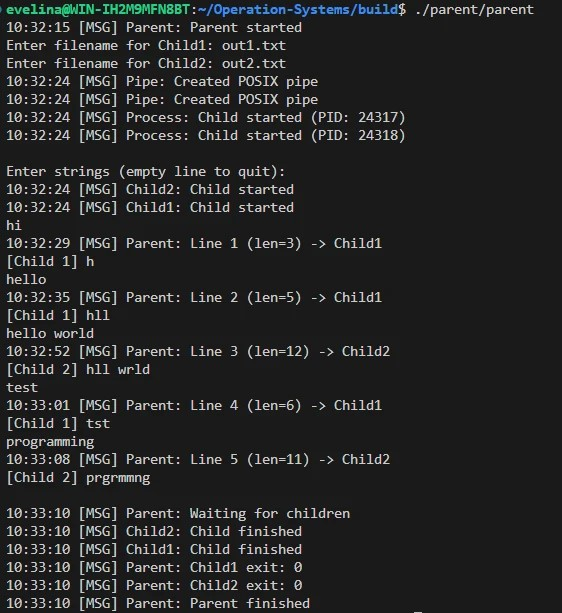
\includegraphics[width=0.95\textwidth]{console.jpg}
    \caption{Консольный вывод программы}
    \label{fig:console}
\end{figure}

Как видно из рисунка 2:
\begin{itemize}
    \item Строки длиной $\le$ 10 символов (\texttt{hi}, \texttt{hello}, \texttt{test}) были отправлены в Child1.
    \item Строки длиной $>$ 10 символов (\texttt{hello world}, \texttt{programming}) были отправлены в Child2.
    \item Гласные буквы успешно удалены: \texttt{hi} $\rightarrow$ \texttt{h}, \texttt{hello} $\rightarrow$ \texttt{hll}, \texttt{programming} $\rightarrow$ \texttt{prgrmmng}.
    \item Оба дочерних процесса завершились с кодом возврата 0.
    \item Родительский процесс корректно дождался завершения детей и завершил работу.
\end{itemize}

На рисунке 3 показано содержимое выходных файлов.

\begin{figure}[h!]
    \centering
    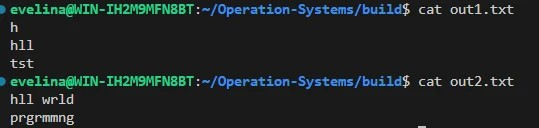
\includegraphics[width=0.95\textwidth]{files.jpg}
    \caption{Содержимое файлов out1.txt и out2.txt}
    \label{fig:files}
\end{figure}

\section*{Выводы}

В ходе выполнения лабораторной работы была спроектирована и реализована модульная система межпроцессного взаимодействия на основе неименованных каналов (pipes). 

При вызове \texttt{fork()} дочерний процесс наследует все файловые дескрипторы родителя. Если не закрыть явно <<чужие>> концы каналов, EOF не придёт, и программа зависнет. Решение этой проблемы путём принудительного закрытия неиспользуемых дескрипторов в дочернем процессе является ключевым для написания надёжных многопроцессных приложений.

Программа спроектирована так, чтобы работать как в Linux, так и в Windows. Для этого системные вызовы POSIX (\texttt{fork}, \texttt{pipe}, \texttt{dup2}, \texttt{waitpid}) инкапсулированы в отдельный файл \texttt{process\_posix.cpp}, а их Windows-аналоги (\texttt{CreateProcess}, \texttt{CreatePipe}, \texttt{WaitForSingleObject})~--- в \texttt{process\_win.cpp}. Бизнес-логика (удаление гласных, маршрутизация строк) остаётся общей и не зависит от ОС. Это помогает экономить время и ресурсы при портировании приложения на другую платформу~--- не нужно переписывать весь код, достаточно реализовать платформенно-зависимый модуль. Система сборки CMake автоматически выбирает нужную реализацию в зависимости от целевой операционной системы.

\end{document}